\documentclass[longbibliography,nofootinbib,twocolumn]{revtex4-1}

\newcommand{\kms}{NuCypher KMS}

\usepackage{listings}
\usepackage{graphicx}
\usepackage{amsmath}
\usepackage[margin=5pt]{subfig}
\usepackage[usenames]{color}

\renewcommand{\baselinestretch}{1.4}
\setlength{\parskip}{1em}
\definecolor{darkgreen}{rgb}{0.00,0.50,0.25}
\definecolor{darkblue}{rgb}{0.00,0.00,0.67}
\newcommand{\figref}[1]{Fig.~\ref{#1}}
\usepackage[breaklinks,pdftitle={NuCypher KMS: Mining}, pdfauthor={Michael Egorov},colorlinks,urlcolor=blue,citecolor=darkgreen,linkcolor=darkblue]{hyperref}
\graphicspath{{pdf/}}

\usepackage[T1]{fontenc}
\usepackage{lmodern}
\lstset{
    basicstyle=\ttfamily,
    basewidth={0.5em, 0.5em},
    columns=fullflexible,
}

\begin{document}

\title{\kms: Mining}

\author{Michael Egorov}
\email{michael@nucypher.com}
\affiliation{NuCypher}

\begin{abstract}
    This paper describes mining mechanisms and economics in \kms.
    It includes inflation rates, mechanisms to incentivise long-term stakers
    and estimates of the number of tokens generated by nodes running in typical modes.
    Also, optimal strategies for stakers who may be affected by market volatility are proposed.
\end{abstract}

\date{\today}
\maketitle

\section{Motivation}

In the future, \kms~will probably be fully paid by network fees.
But initially, when the adoption isn't yet high, miners who run the nodes necessary for network operation and keep re-encryption keys,
will need to be subsidised.
This will be done through an inflation schedule, where all the inflation is given back to miners.

Distribution of rewards should have the following properties:
\begin{itemize}
    \item All the inflation is distributed to stakers who run the nodes, proportionally to their stake;
    \item The amount of work (and, hence, fees earned) is proportional to stake;
    \item Stakers are incentivized (by a higher reward rate) to run long-term nodes;
    \item High inflation doesn't depreciate the price in order to keep liquidity for new stakers;
    \item Stakers are incentivized to stay online all the time.
\end{itemize}

In the paper we address all these points, calculate expected earnings of miners who run nodes and devise optimal mining strategies.

\section{Historical examples of inflation}

Let's review inflation schedules of different cryptocurrency projects:
DASH~\cite{dash:whitepaper} and ZCash~\cite{zcash}.

DASH has a hybrid of Proof-of-Work (POW) and Proof-of-Stake (POS).
It has $45\%$ of inflation going to POW miners, $45\%$ to staking master nodes, and $10\%$ reserved for budget proposals~\cite{dash:emission}.
After the first year, its emission was $18.42\%$ APR, decreasing by $1/14$ every $383$ days.
With this setting, $60\%$ of DASH coins are locked in masternodes for staking, according to the node statistics.
It's unclear how inflation rate affects the price (and if it does here), but the useful data point is that there are $60\%$ of coins locked for staking.
Perhaps, that is something to expect in a network where staking is an option.

% TODO: replot in a more reasonable shape
\begin{figure}
    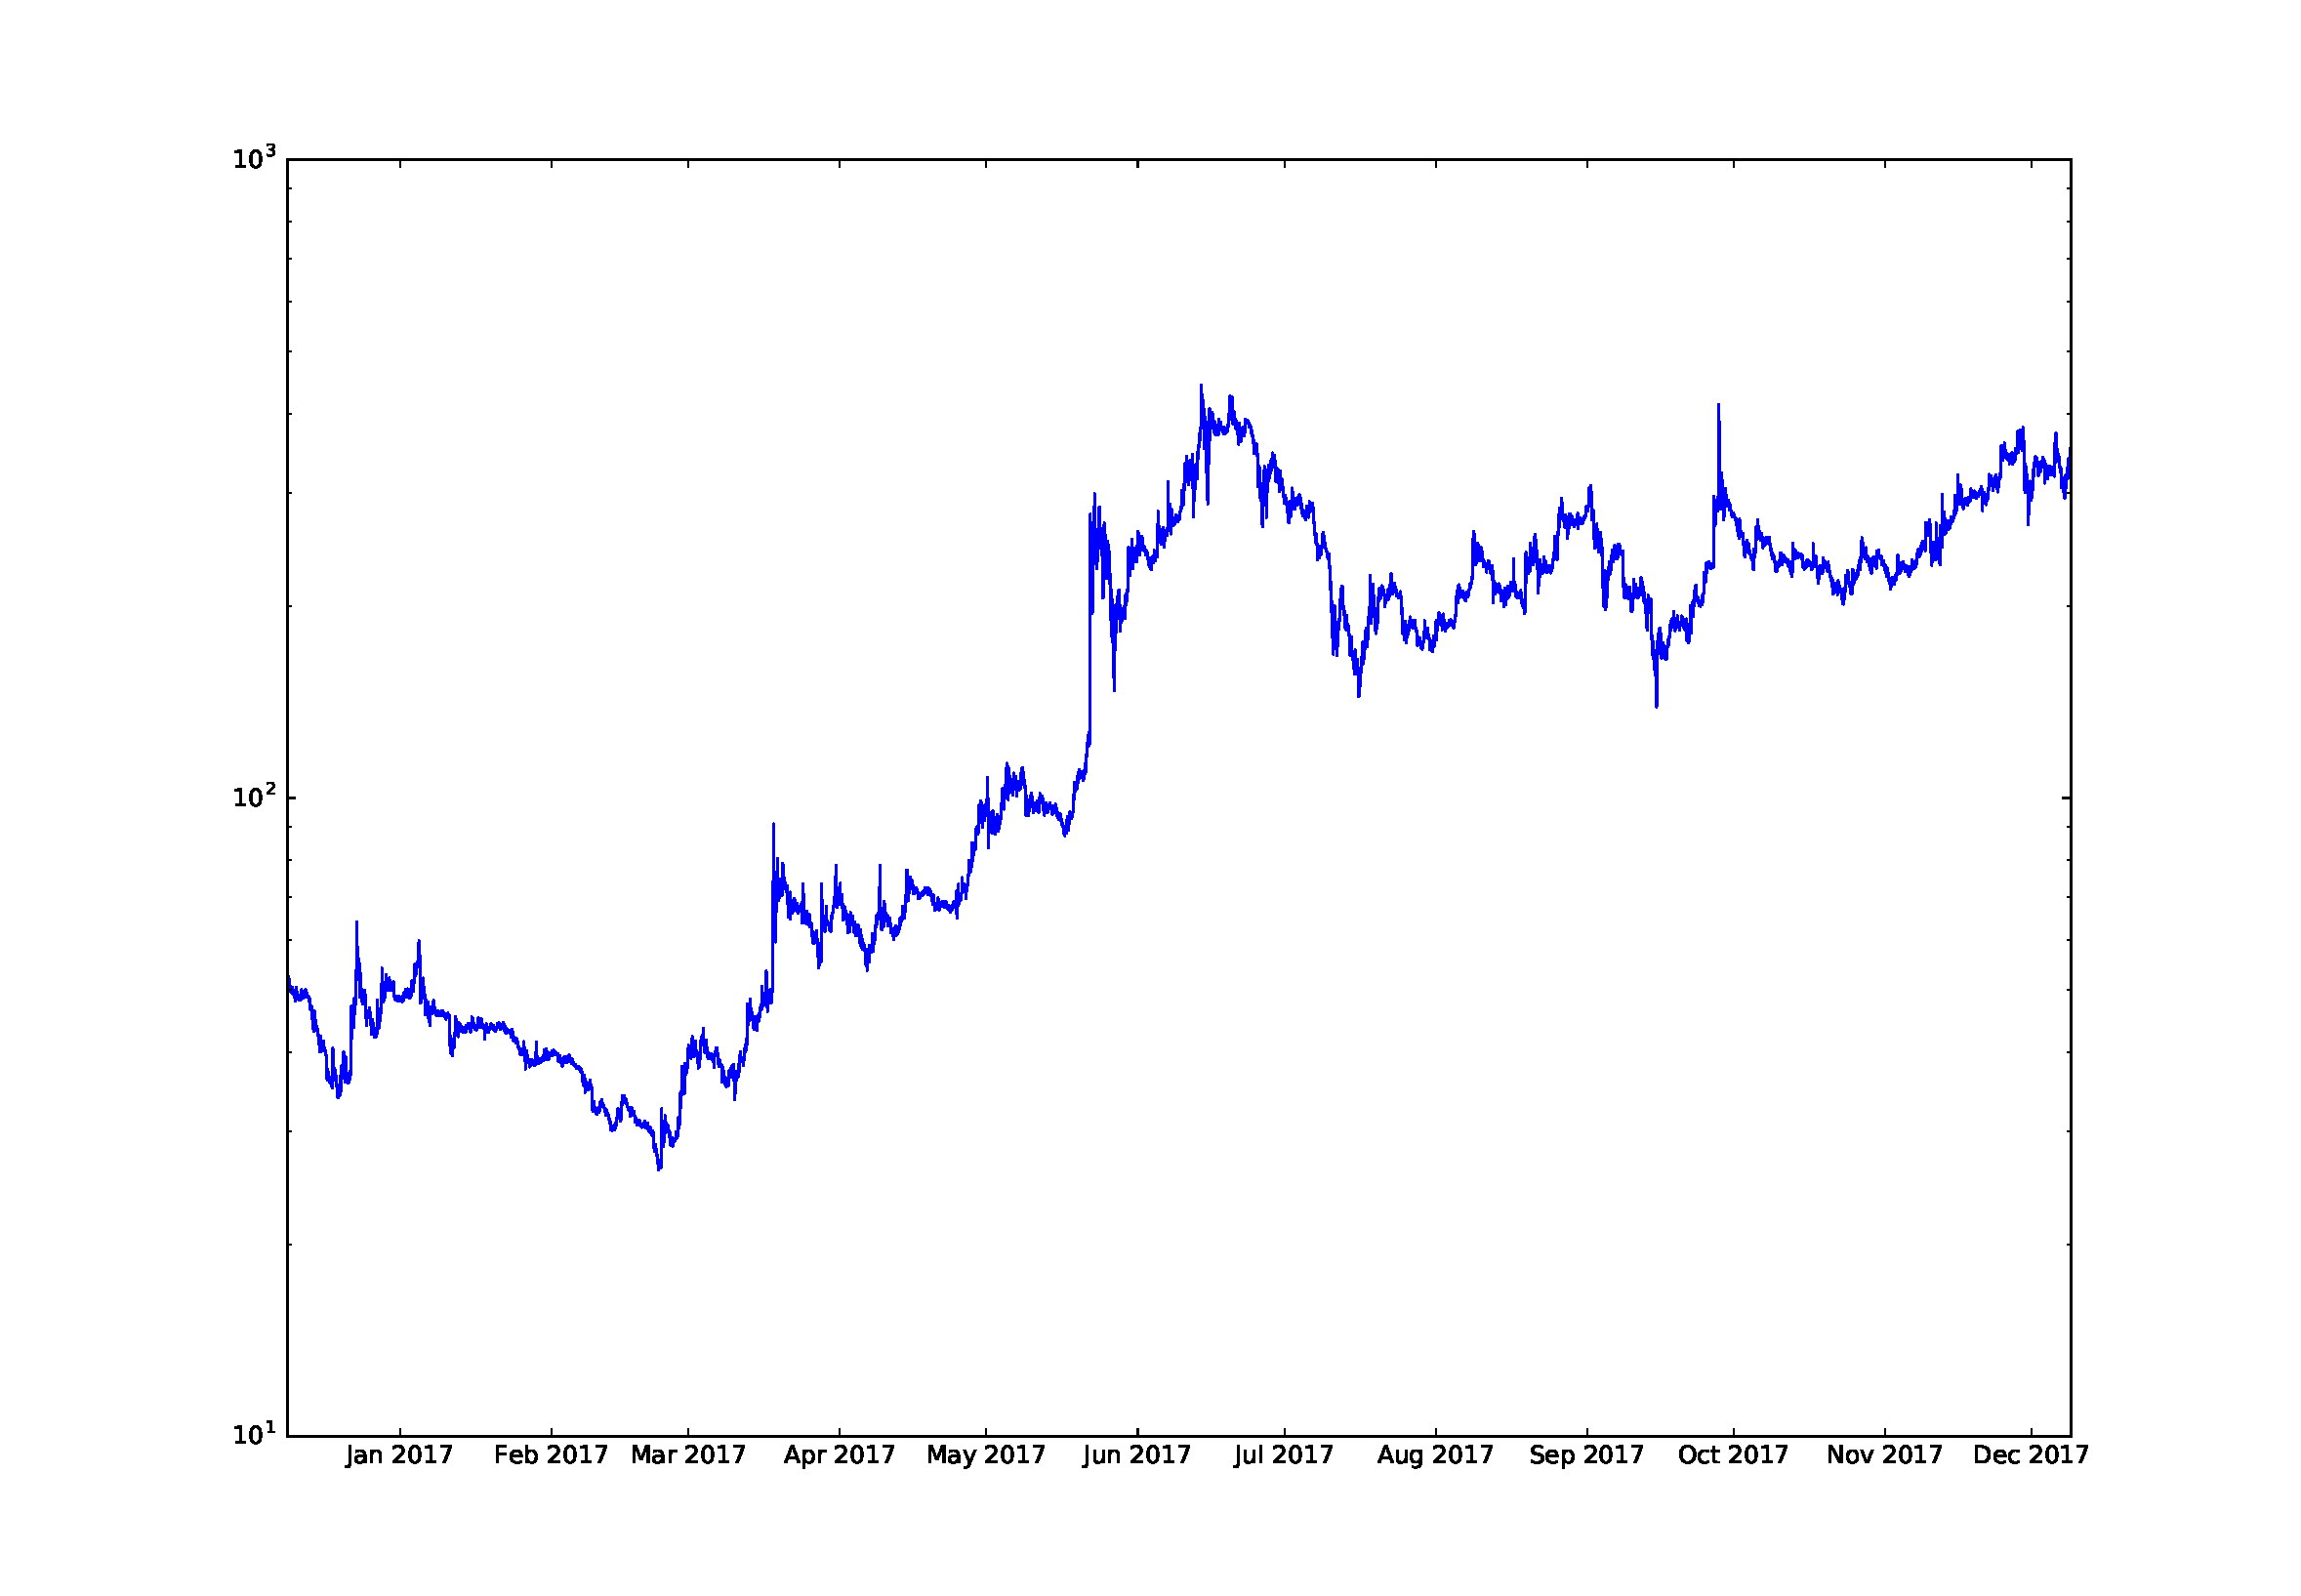
\includegraphics[width=\columnwidth]{pdf/zcash-price.pdf}
    \caption{Historical price of ZCash in logarithmic scale. Note the minimum at 23 Feb 2017}
    \label{fig:zec}
\end{figure}

ZCash is very interesting because it started with an extremely high inflation rate.
This caused a short-term price drop (even though the market capitalization was growing)~(\figref{fig:zec}).
But at some point (23~Feb~2017), the price started going up.
ZCash block rewards yield $50$~ZEC every $10$~min, and ZEC supply at Feb~23 was $727$k~ZEC.
This corresponds to $360\%$~APR.
It is even more remarkable given the fact that miners who mined ZEC are probably those who dump and exchange the proceeds into something else (and also pay
electricity bills).
This gives us information about what would be the maximum allowable inflation which still doesn't create too much downward pressure on the price.

\section{Mining protocol}

A miner commits to stay available for at least time $T$.
For that, he or she specifies the unlocking time $t_1$.
Minimal lock time $t_1 - t$ should be not less than $T_{\min} = 1$~month.
Number of coins locked for staking $l$ should be no less than some value $S_{\min}$.

\begin{figure}
    \subfloat[Unlocking in a single step]{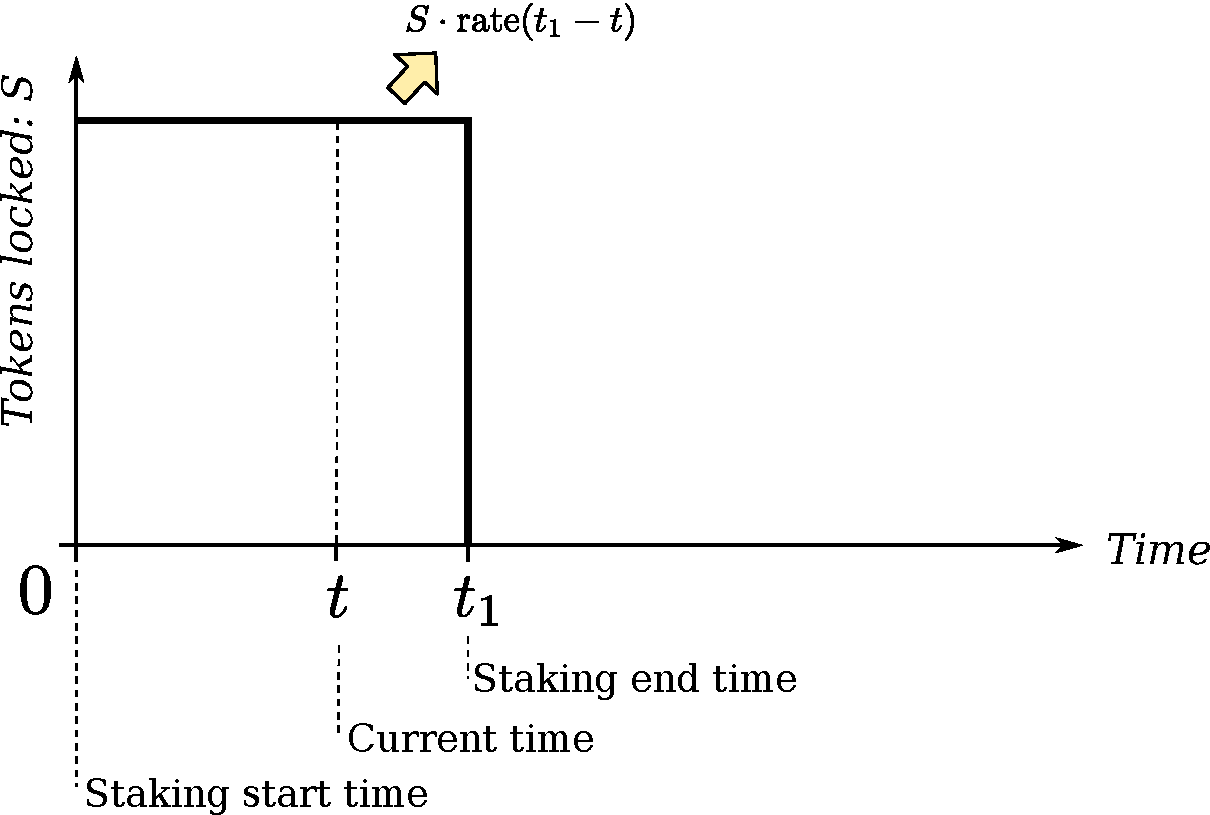
\includegraphics[width=\columnwidth]{pdf/one-step.pdf}}\\
    \subfloat[Splitting into two steps]{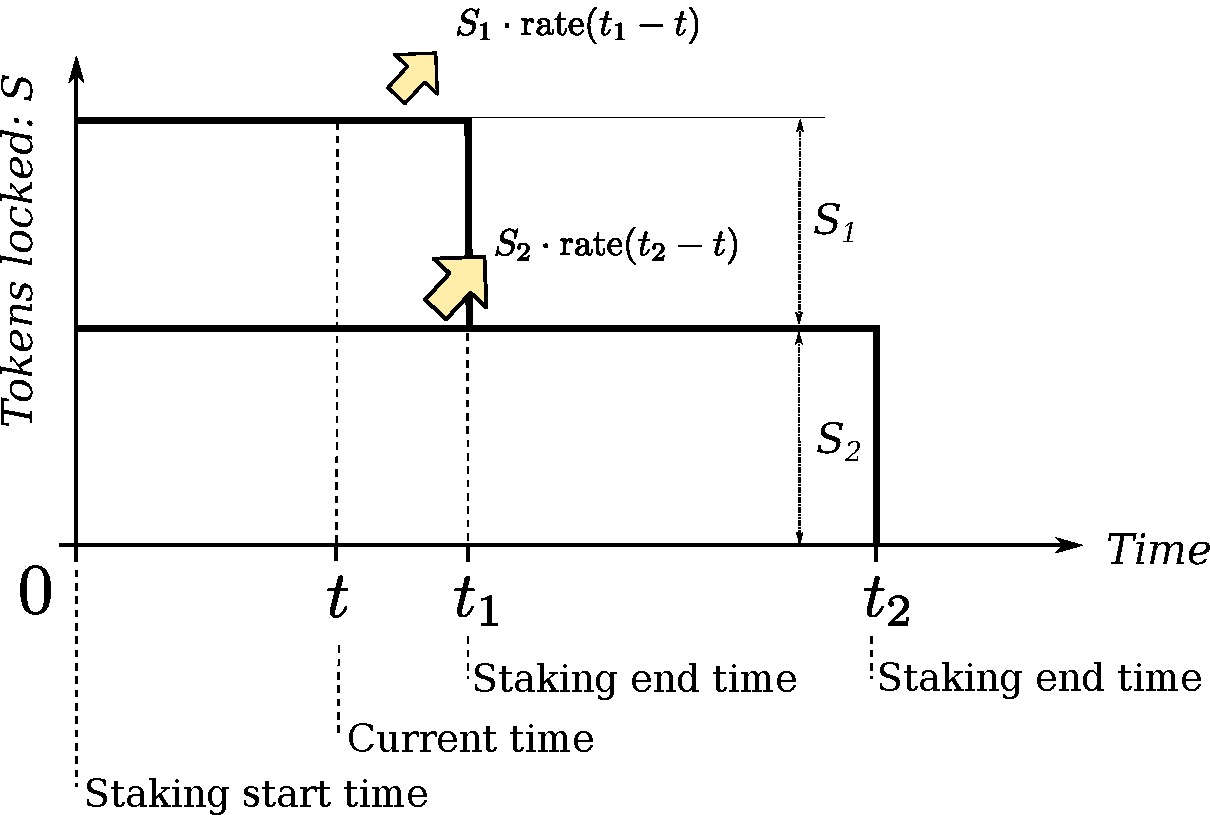
\includegraphics[width=\columnwidth]{pdf/two-steps.pdf}}
    \caption{
        When staked, an unlock time $t_1$ is specified.
        At any time the unlock time can be increased (but not decreased).
        The stake can optionally be split into two parts where only one part is extended till $t_2$.
    }
    \label{fig:mining-modes}
\end{figure}

At any point a miner can split his stake or any piece of his stake into two pieces~(\figref{fig:mining-modes}).
The size of each piece should be not less than $S{\min}$.
The reason for the possibility of that splitting is dependence of reward rate on the lock time $T$, which we'll discuss later.
At any point the miner can increase (but not decrease) $T$ and add more coins to stake.

\section{General inflation properties}

\subsection{Initial inflation}

Let's assume that we'll have the same number of tokens locked as DASH: $\lambda=60\%$.
Then we'll have $1-\lambda=40\%$ in circulation.
If we have inflation rate $I$, then adjusted inflation rate (e.g. inflation as if the locked tokens didn't exist) of tokens in circulation will be:
\begin{equation}
    I^* = \frac{I}{1-\lambda},
\end{equation}
and we should be comparing $I^*$ with historical examples of inflation.
If we take $I^*=350\%$ (turnover point of ZCash price in an overall bullish market), the corresponding inflation $I$ will be $140\%$~APR.

To be on the safe side, we choose the starting inflation to be $I_0=100\%$~APR (or, in other words, $1/365$ per day).

\subsection{Inflation decay}

Initially, the inflation subsidises mining, but payments for re-encryption services will generate the majority or all the revenues of miners in the long run.
If all miners have the same, maximum reward rate, we choose the inflation rate to decay by factor of $2$ in $T_{1/2} = 2$ years.
The inflation, depending on time passed from the Genesis $t$, looks like:
\begin{equation}
    I(t) = I_0 \cdot 2^{-\frac{t}{T_{1/2}}} = I_0 \exp\left[ -\ln{2} \frac{t}{T_{1/2}} \right].
\end{equation}
In this case, the dependence of the token supply on the time $t$ is:
\begin{equation}
    \label{eq:supply-time}
    S(t) = S_0 + \int_0^{t} I(t)\, dt = S_0 + \frac{I_0 T_{1/2}}{\ln{2}}\left[1 - 2^{-\frac{t}{T_{1/2}}} \right],
\end{equation}
Let's call relative initial annual inflation $i_0$, and then $I_0 = i_0 S_0$.
For $100\%$~APR, $i_0=1$ and $I_0=S_0$~per~year, and the maximum number of tokens which will ever be created is:
\begin{equation}
    S_{\max} = S(\infty) = S_0\left(1 + \frac{i_0 T_{1/2}}{\ln{2}}\right) \approx 3.89\, S_0,
\end{equation}
where $S_0$ is initial number of tokens.

\subsection{Implementation of the exponential decay in a smart contract}

Complex functions like exponentials, if implemented in smart contracts, would be quite costly.
Fortunately, the exponential is a solution of a differential equation where inflation is proportional to the amount of not yet mined tokens:
\begin{eqnarray}
    I(t) &=& \frac{\ln{2}}{T_{1/2}} \left( S_{\max} - S(t) \right)\\
    dS &=& I(t)\, dt,
\end{eqnarray}
where $S(t)$ is the current token supply with $S(0)=S_0$ and the time step $dt$ can actually be equal to the mining period ($1$~day).
Each mining node can trivially calculate its $dS$ in a smart contract using very few operations and the coin supply $S$ from the last period.
So, the amount of tokens mined for the node $i$ and the time period $t$ will be:
\begin{eqnarray}
    \label{eq:rate-max}
    ds_{i,t} &=& \frac{l_i}{L} \frac{\ln{2}}{T_{1/2}} \left( S_{\max} - S_{t-1} \right),\\
    dS_t &=& \sum_i ds_{i,t},
\end{eqnarray}
where $l_i$ is the number of tokens locked by the miner $i$, $L$ is the total number of tokens locked.
Instead of calculating all the sum over $i$, each miner $i$ can add her portion $ds_{i,t}$.

\subsection{Mining rate and staking time}

\begin{figure}
    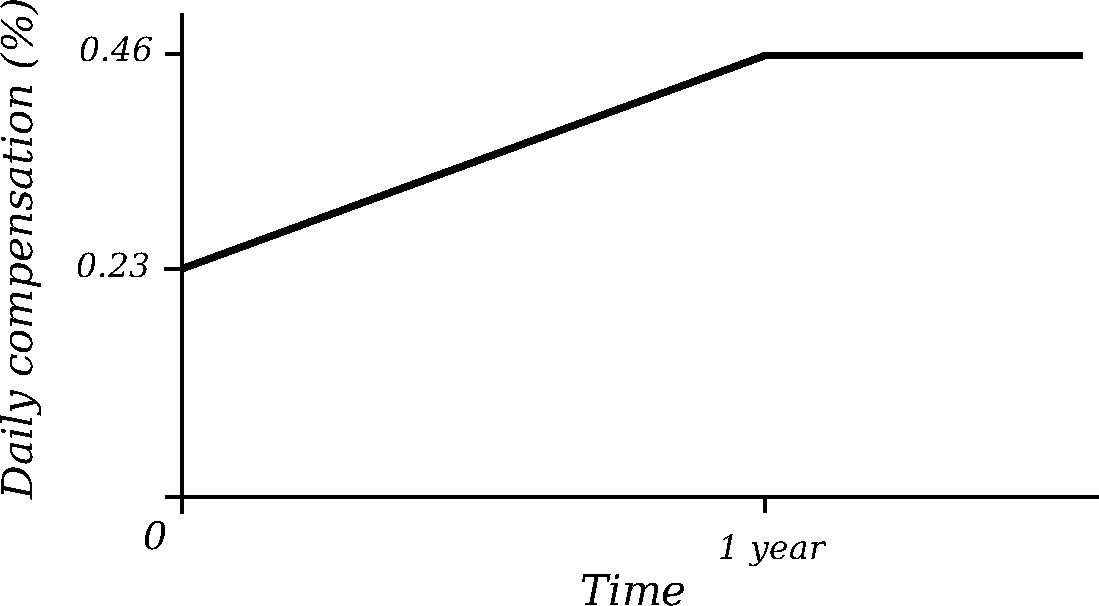
\includegraphics[width=\columnwidth]{pdf/rate.pdf}
    \caption{Dependence of the compensation rate on staking duration. We assume $60\%$ of all tokens locked for staking}
    \label{fig:reward-rate-vs-duration}
\end{figure}

We want to incentivize miners to keep serving re-encryption policies for at least $1$~year.
However, short-term stakers are still useful and should be rewarded.
We will give the full compensation ($\kappa=1$) to the stakers who are committed to stake at least $T_1=1$~year,
however those who stake for $T_{\min}=1$~month will get close to half the compensation ($\kappa\approx0.54$) (\figref{fig:reward-rate-vs-duration}).
The individual daily compensation rate for a miner looks as:
\begin{eqnarray}
    \kappa &=& \left(0.5 + 0.5\frac{\min(T_i, T_1)}{T_1}\right)\\
    T_{i,\text{initial}} &\ge& T_{\min},\\
    \delta s_{i,t} &=&  \kappa\, \frac{l_i}{L} \frac{\ln{2}}{T_{1/2}} \left( S_{\max} - S_{t-1}\right).\\
\end{eqnarray}
The unlocking time $T_i$ means the time left to unlock the tokens $t_1 - t$.
The initial $T_i$ cannot be set smaller than $1$~month,
but it eventually becomes smaller than that as the time goes on, and the miner gets close to unlocking the stake.

This has implications on the global token economy.
Firstly, if stakers, despite smaller compensation, prefer to stake for shorter, that creates smaller daily token supply.
Since this usually should coincide with bear market, reducing the issuance during that time sounds like a good idea.

Interestingly enough, $\kappa < 1$ prolongs the compensation half-decay time $T_{1/2}^* = T_{1/2} / \kappa^*$, where $\kappa^*$ is the mean staking parameter.
If all the stakers have $\kappa^* = \kappa = 0.5$, this prolongs $T_{1/2}$ to be $4$~years instead of $2$.

The total supply over time (Eq.~\ref{eq:supply-time}) at $\kappa^* \ne 1$ will then look like:
\begin{equation}
    \label{eq:adjusted-supply-time}
    S(t) = S_0 \left[1 + \frac{i_0 \kappa^* T_{1/2}^*}{\ln{2}}\left(1 - 2^{-\frac{t}{T_{1/2}^*}} \right) \right].
\end{equation}

\section{Mining strategies and expected compensations}

In this section, we look at three possibilities: miner taking all the block rewards, miner adding all the compensation to what's currently staked and miner spinning
the node down to get all the tokens unlocked after the time $T$ (as well as the rewards).
Every of these possibilities could have different distributions of $\kappa$.
Let's consider $\kappa=1$ and $\kappa=0.5$ as two marginal values.
Let's take amount of tokens locked to be $\lambda=60\%$, as in DASH.
We'll plot graphs of daily rewards, as well as calculate the rewards during the first year in each of these scenarios.

\subsection{Withdraw mining compensation}

This is the simplest case.
The total amount of tokens staked in the network can be expressed as $L=\lambda S$.
The amount of stake stays constant in this case and equal to $s_i = l$, and the mining rate (e.g. the cumulative rewards) is:
\begin{equation}
    \frac{dr}{dt} =  \kappa\, \frac{l}{\lambda S(t)} \frac{\ln{2}}{T_{1/2}} \left( S_{\max} - S(t)\right).
\end{equation}
When we substitute $S(t)$ from Eq.~\ref{eq:adjusted-supply-time} and integrate over time, we find total rewards:
\begin{equation}
    r(t) = l \frac{\kappa}{\kappa^* \lambda} \ln\frac{S(t)}{S_0}.
\end{equation}

If $\kappa=1$ (staking for $1$~year+) and $\lambda=60\%$ ($60\%$ of all nodes in the network are staking),
miner's compensation starts from $0.46\%$~per~day in NKMS tokens,
or $100.2\%$ during the first year of staking.

We should note that if other miners stake for less than a year ($\kappa^* < 1$), the inflation rate decays slower, and the compensation over a given period
will be higher.

\subsection{Restake mining compensation}

Instead of taking all the mining compensation, it could be restaked into the node in order to get even more jobs and, provided that the hardware is maintained
powerful enough to cope with those, get even higher compensation.
In this case, the actual stake $l$ is constantly increasing with time:
\begin{equation}
    \frac{dl}{dt} =  \kappa\, \frac{l}{\lambda S(t)} \frac{\ln{2}}{T_{1/2}} \left( S_{\max} - S(t)\right).
\end{equation}
If we substitute $S(t)$ from Eq.~\ref{eq:adjusted-supply-time} and solve this differential equation against $l$, we get:
\begin{equation}
    l(t) = l(0)\,\left[ \frac{S(t)}{S_0} \right]^{\frac{\kappa}{\kappa^* \lambda}}.
\end{equation}
If $\kappa=1$ (staking for $1$~year+) and $\lambda=60\%$ ($60\%$ of all nodes in the network are staking),
miner's compensation starts from $0.46\%$~per~day in NKMS tokens,
or $l(1) - l(0) = 177.5\%$ during the first year of staking.

\subsection{Take mining rewards and spindown}

When the node spins down, the miner doesn't extend the time for end of staking $t_1$,
and rewards are constantly decreased because the time left to unlock becomes smaller and smaller,
effectively decreasing $\kappa$ gradually towards $0.5$.
That's the default behavior: to avoid that, the miner should set $t_1$ large enough, or increase $t_1$ periodically.

\subsection{Edge case: connection problems}

If the miner is found to be non-operational and/or cannot confirm the activity, the tokens aren't unlocked during the mining period when that happens (and the
rewards aren't mined).
It's not too bad for the miner if that happens, however one cannot lock tokens for mining and get them unlocked, even without getting staking rewards.
So if the miner commits to stake for at least a year, it implies a year of operation.

The ``connection problems'' may also be the time when the miner upgrades the software, which is an absolutely legitimate reason to be offline for a short time.

\section{TLDR}

\subsection{How much will I be earnining if I run a node}
It depends on how early you start (the earlier, the better), and for how long you commit to provide re-encryption services.
If you commit to work for $1$~month, you'll be getting approximately $54\%$ of what you'll be getting if you commit for $1$~year or more.
Also the compensation is inversely proportional to the total amount of tokens staked by all the participants.
Finally, if you choose to automatically add the tokens earned to the stake, this will increase the rewards because your stake will be increasing as well.

For example, if $60\%$ of tokens in the system are always staked, you'd be earning $0.46\%$ in day $1$.
With this amount of stakers, if you withdraw all the earned tokens instead of re-staking them, in the first year you'd earn $100.2\%$ of your stake.
But if you restake all your tokens, in the same first year you'd earn $177.5\%$ of the tokens you staked.

\subsection{How many tokens will be in the existence}
We'll start with $1$~billion tokens, and the maximum amount of tokens ever mined will be $3.89$~billions.

\subsection{What's the inflation rate}
The inflation rate will depend on how many short-term miners and long-term miners are in the system.
Depending on this, the initial inflation will be between $50\%$~APR (when all miners are very short term) and $100\%$~APR (when everyone commits for a long
term).
The inflation will be decaying exponentially every day, halving in time between $2$~years (when all the miners are long term)
and $4$~years (when all the miners are short term).

\bibliography{mining-paper}

\end{document}
